\section{Results}
The actors of open and reproducible data science leave traces of their timestamped contributions on online social coding platforms. The scientists, who participated to the Astro Hack Week (AstroWeek), used GitHub. Thus, we could extract their detailed activities before, during and after the AstroWeek. Since they also kept records of their activities, on the AstroWeek blog, on Twitter, and other social media platforms, we could pull out ethnography material, which further informs on the context of the AstroWeek community building. Here, we show how the AstroWeek has been an significant impulse for the community, with long-term spillovers, which may only partially related to projects developed during the AstroWeek. Recognizing that while the AstroWeek is an opportunity for lay participants, it may be perceived as a disruption for seasoned data scientists who invested time teaching open and reproducible science, we measure how the distribution of contributions per actor changes during the AstroWeek.


\begin{figure*}[!t]
\centering
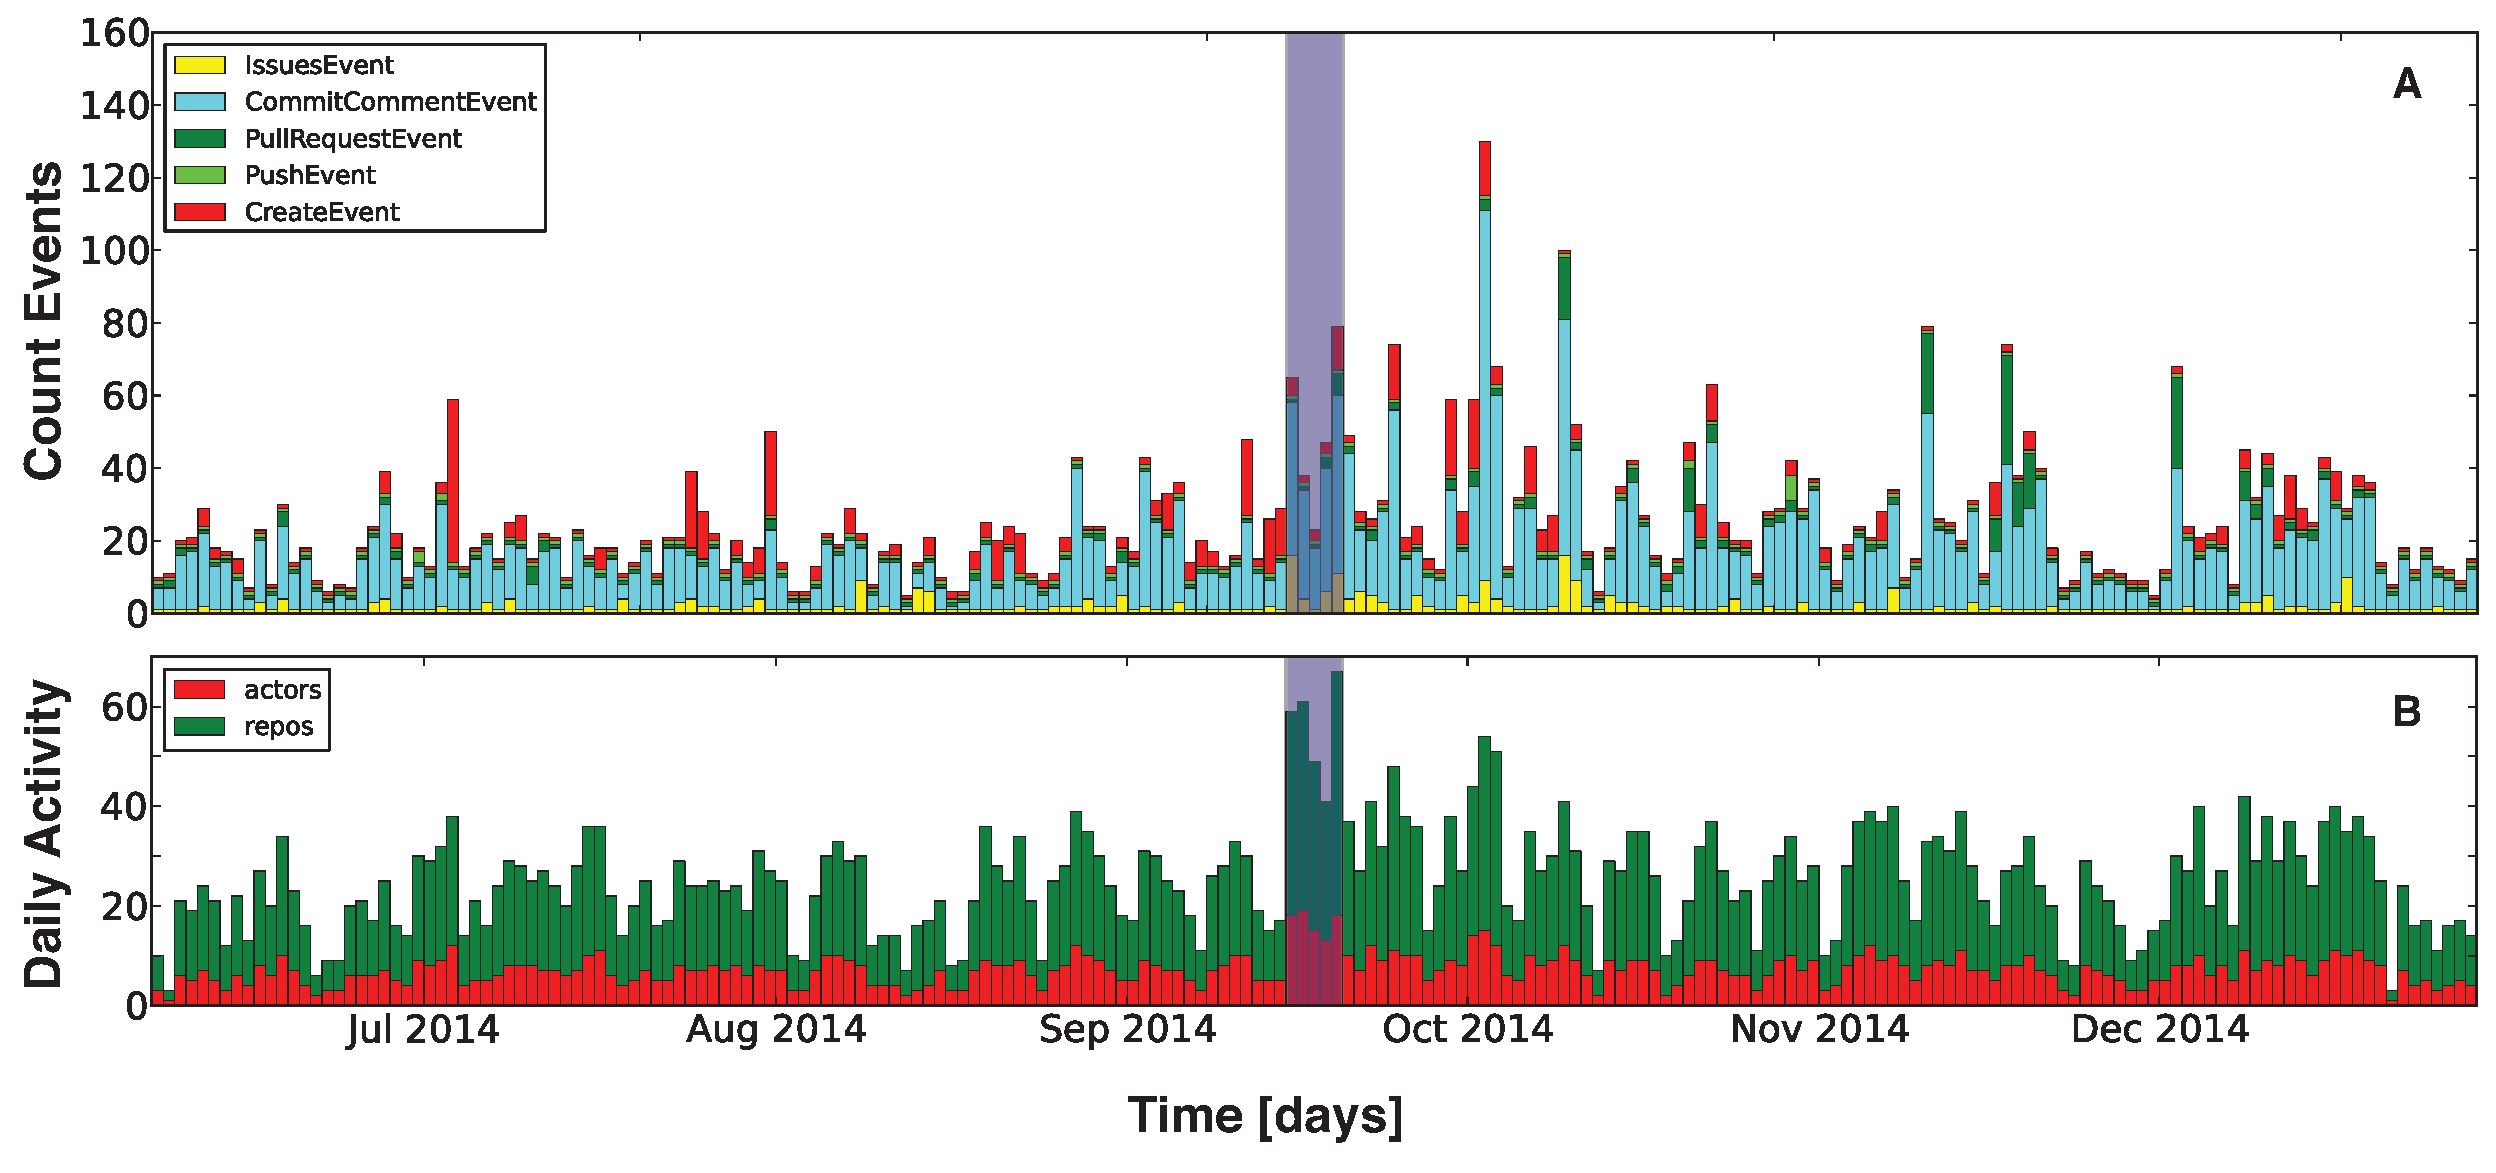
\includegraphics[width=2.0\columnwidth]{figures/timeline.eps}
\caption{ {\bf Panel A:} Histogram of daily events stacked by type, as described by the legend. The shaded purple area highlights the Astro Hack Week. {\bf Panel B:} (Stacked) daily activity of actors and repositories. The daily count of events, as well as actor and repo activity exhibit a burst during the AstroWeek, with an increase of respectively 60\%, 87\%, 53\%, compared to the average daily activity in the last 6 months before. This burst is followed by a slow decay until the end of december 2014.
%For daily active actors {\bf [repos instead?]}, the median, 75th and the 90th percentiles are reported. During the AstroWeek all days have an actor activity above the 90th percentile {\bf [Note that there is an obvious selection bias here, because we precisely study this community $\rightarrow$ it remains to be clarified why it's relevant to report this value]}, and the number of events is above the 75th percentile 4 days out of 5. While bursts of events are not rare, the coalescence of actors (and of repos), is unique over the year around AstroWeek, and shows the unique ``dynamics occurring during, and after this community building event."
}
\label{fig:time_series}
\end{figure*}

\subsection{The Astro Hack Week Impulse}
Figure \ref{fig:time_series} shows the number of events by type (panel {\bf A}), and the number of active contributors and active repositories per day (panel {\bf B}), for the 30 participants with a GitHub account. During the AstroWeek, the daily count of active participants, active repositories and events, increased by respectively $84.3\%$, $50.7\%$, and $58.4\%$. The number of new repositories created jumped from a weekly average of 7.5 (since March, 15, 2014) to 43 repositories created during the hackathon. The number of repository creations remained then sustained for nearly one month (yellow bars), showing that even after the end of the meeting, former participants have created and worked on new data science tools, beyond the initial scope. After the peak, the activity (in terms of events, active actors, or repositories) also exhibits a sustained --yet decaying-- activity until roughly 100 days after the hacking week. These slow decays are expected from empirical results in open source software communities \cite{sornette2014much}, and from the theory \cite{saichev2013hierarchy}. They are key to rationalize and measure the after-effects of the Astro Hack Week.


\subsection{Long-Memory Process and Slow Activity Decay}
To better grasp these long-term and slow decaying dynamics of activity --directly and indirectly related to the AstroWeek-- we investigated decays, first considering only repositories created during the hackathon week \cite{astro_hackpad} and from \cite{astro_github}, and then all repositories created by the community after the AstroWeek.

Figure \ref{fig:decay_astro_repos} shows the relaxation of activity directly related to the Astro Hack Week, over the 100 days following $t_0$, i.e., September 15th, 2014. In double logarithmic scale, we observe negative linear slopes, which confirm the power law relaxation after an exogenous shock, given by equation (\ref{eq:critical_decay}). The decay exponents $\alpha$ for daily count of active actors and contributed repositories are similar ($alpha = 0.60\pm0.08$), while the number of events per day decays faster, with exponent $0.87\pm0.14$, yet from a higher peak (close to 100 events at $t_0$). The average decay of number of events per actor (resp. repository) is obtained as $\sim 1/(t-t_0)^{\beta}$ with $\beta \approx (0.87 - 0.60) = 0.27$. Thus, after 100 days, the activity per actor (or per repository, since in both cases $\alpha \approx 0.60$), is still $30\%$ of the activity per actor at $t_0$. At the same time ($t=100$), the number of actors active on repositories created during the AstroWeek is only $6.30\%$ of its peak activity, and the number of events is nearly $1.8\%$ of initial activity (i.e., roughly 100 events per day). In other words, the activity directly related to the AstroWeek has become nearly residual after 100 days.

We now turn to activity un-conditioned (i.e., not directly related to the Astro Hack Week), but triggered by the community building effect. Figure \ref{fig:relaxation} shows the relaxation of activity (again in double logarithmic scale) over the 100 days following the AstroWeek. We observe negative linear slopes, which confirm again the power law relaxation given by (\ref{eq:critical_decay}) after $t_0$. For daily events, actors and repository activity, the exponents $\alpha$ are roughly the same (respectively $0.28\pm0.08$, $0.22\pm0.05$,$0.21\pm0.05$). The un-conditioned decay, in comparison with Figure \ref{fig:decay_astro_repos}, is much smaller. For the matter of illustration, taking $\alpha = 0.25$, the remaining activity after $100$ (resp. $1000$, $10^5$) days, is $31.6\%$ (resp. $17.8\%$, $10\%$) of the initial peak activity. Thus, in theory, even after an arbitrary long period, the follow-up activity triggered by the AstroWeek is likely to remain significant. For instance, after $100$ days (resp. $1,000$ days), $13$ (resp. $7$) out of $43$ average daily events, i.e., $30\%$ (resp. $16\%$), may be considered as direct and indirect follow-up events of the AstroWeek. 

The apparent long-term influence of the the Astro Hack Week is remarkable, and deserves further scrutiny, in order to identify its origins. Figure \ref{fig:relaxation} shows also the decay of the weekly count of repository creations (black circles). Yet the decay follows a much faster power law relaxation with exponent $0.60\pm0.10$ -- compared to the daily count of actors, repositories, and events -- its after-effects are not negligible, considering that each repository triggers follow-up activity. If we consider that creating a repository is an originating event, from which events are triggered, hence generating follow-up activity from one or several actors, then, we can interpret the slow-decaying dynamics of the AstroWeek as the combined effect of an exogenous critical triggering of repositories and the long-memory decay of activity of repository created. {\bf [here, I could do a quick numerical verification that these repositories, indeed trigger events]}. 

%follows: repositories are created following $\sim A_{t_0}/(t-t_0)^{\alpha}$ with $\alpha \approx 0.6$. {\bf [I think this is wrong : ``Then, each repository triggers activity on average as $\sim 1/(t-t{0})^{\gamma}$ with $\gamma \approx 0.6 - 0.28 = 0.32$." $\rightarrow$ here, there is a special renormalization of the exponent $\rightarrow$ We shall maybe not enter here in this paper]}.

%{\bf [Say something on super-linear productive bursts, and the fact that the Astro Hack Week looks like a burst, yet with a similar structure of contributions?]} 

%What has changed after these 100 days? look at activity resume after Holidays (i.e., January 15th) ?  {\bf [End of year should be considered as a sufficiently significant event]}.


\begin{figure}[!t]
\centering
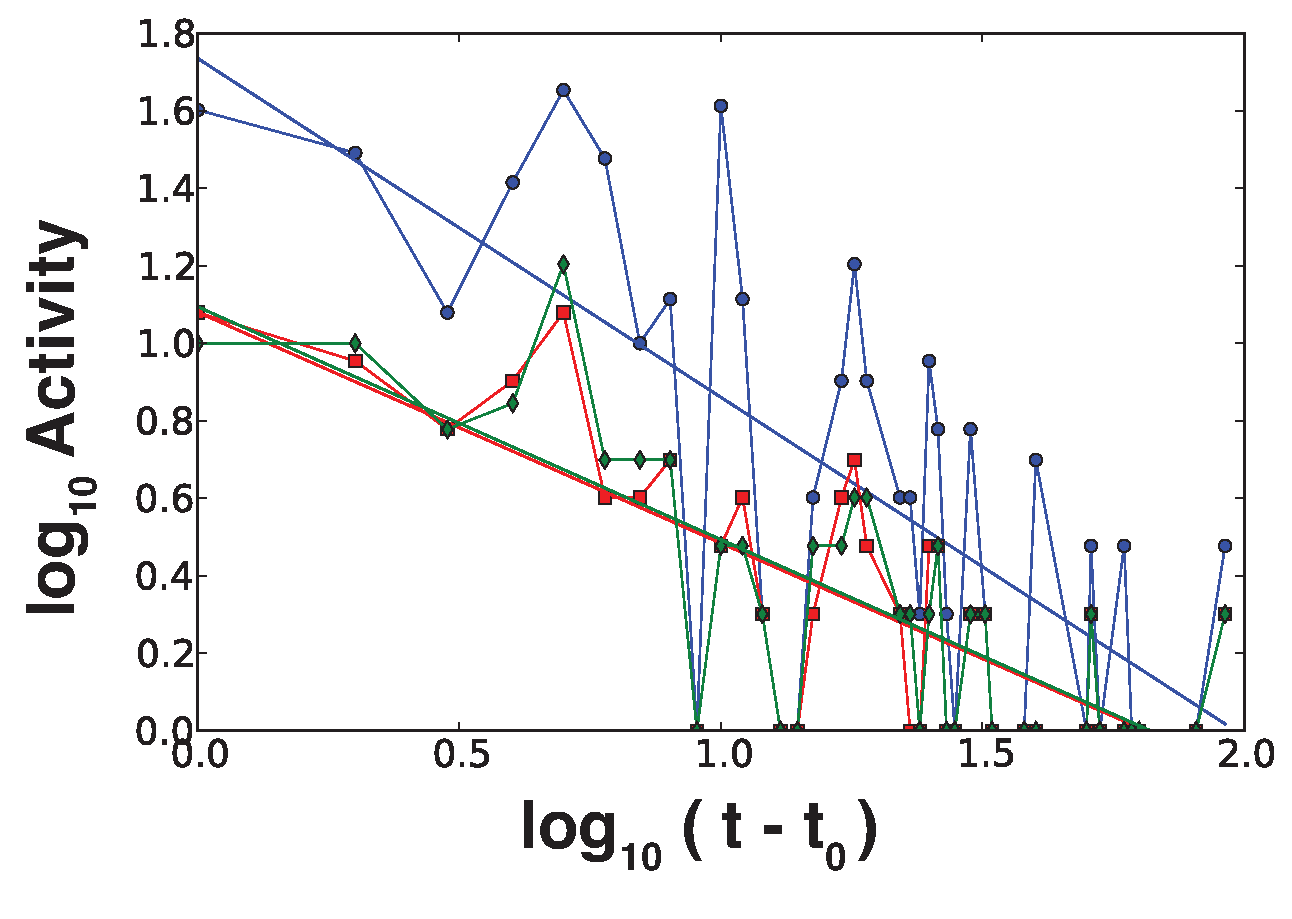
\includegraphics[width=0.9\columnwidth]{figures/relaxation_aw_repos.eps}
\caption{Decay (in double logarithmic scale) of daily activity on Astro Hack Week repositories only: actors (red), repositories (green), and events (blue). All activity types are fitted with power law decay following formula (\ref{eq:critical_decay}), with very similar exponents for actors, and repositories ($alpha = 0.6\pm0.08$). The relaxation of the daily events is much faster with exponent $0.87\pm0.14$. Comparison with Figure \ref{fig:relaxation} shows that actors, have rapidly started to work on other repositories, slightly less related to the Astro Hack Week, yet they have not abandoned the projects started during the period Sept. 15--20, 2014.}
\label{fig:decay_astro_repos}
\end{figure}

\begin{figure}[!t]
\centering
\includegraphics[width=0.9\columnwidth]{figures/relaxation.eps}
\caption{Decay (in double logarithmic scale) of daily activity after the start of the Astro Hack Week ($t_0 = $ september 15th, 2015): actors (red), repositories (green), events (blue) and weekly creation of repositories (black circles). All activity types are fitted with power law decay as formula (\ref{eq:critical_decay}), with very similar exponents $alpha$ for actors, repositories and events: respectively $0.22\pm0.05$, $0.21\pm0.05$, and $0.28\pm0.08$. The decay of created repositories is however faster with exponent $0.60\pm0.10$.}
\label{fig:relaxation}
\end{figure}


\subsection{Reorganization of the Distribution of Contributions}
From \cite{sornette2014much}, we know that the number of events $R$ per time window is a super-linear function,

\begin{equation}
R \sim c^{\beta}
\label{eq:superlinear}
\end{equation}

with $c$ the number of active contributors and $\beta$ the scaling exponent typically found $\beta \approx 4/3$ in a large number of open source software projects. This law of super-linear production stems from critical cascades of individual and collective contribution events. In the case of individual contributions, cascades, lead heavy-tailed distributions (i.e., large deviation) of individual contributions. In other words, the super-linear effect observed is largely due to a few large contributors. Figure \ref{fig:tradeoff} (panel {\bf A}) shows that super-linear productive bursts of events have also occurred on a regular basis, within the AstroWeek community, before, during and after the hackathon.

However, the AstroWeek gathered both lay and seasoned data scientists. Questioned on the trade-offs implied by spending time teaching lay participants, a senior contributor (P4) answered that the AstroWeek prevented him from contributing as much as what he would routinely do. Figure \ref{fig:tradeoff} (panel {\bf B}) shows a comparison of event counts per actor during and after the AstroWeek as a function event counts per actor before the hackathon (in double logarithmic scale). While the relation between counts before and after is almost linear (scaling exponent $= 0.82\pm0.10$ close to $1$), the comparison of event counts during the AstroWeek as a function as before exhibits a scaling with $\mu = 0.35\pm0.08$, which is strongly sub-linear. In other words, while largest contributors before AstroWeek are still the most contributing actors during the AstroWeek, the number of their contributions is marginally decreasing, confirming the statement provided by interviewee P4. Yet contributions remain bursty during AstroWeek, so events not contributed by senior actors, seem to be --at least partly-- compensated by less senior actors. This contribution gap may be further identified by considering that while the number of daily active participants increased by $84.3\%$ during the AstroWeek, the number of events increased by only $58.4\%$ (also clearly visible on Figure \ref{fig:time_series}).

\begin{figure}[!t]
\centering
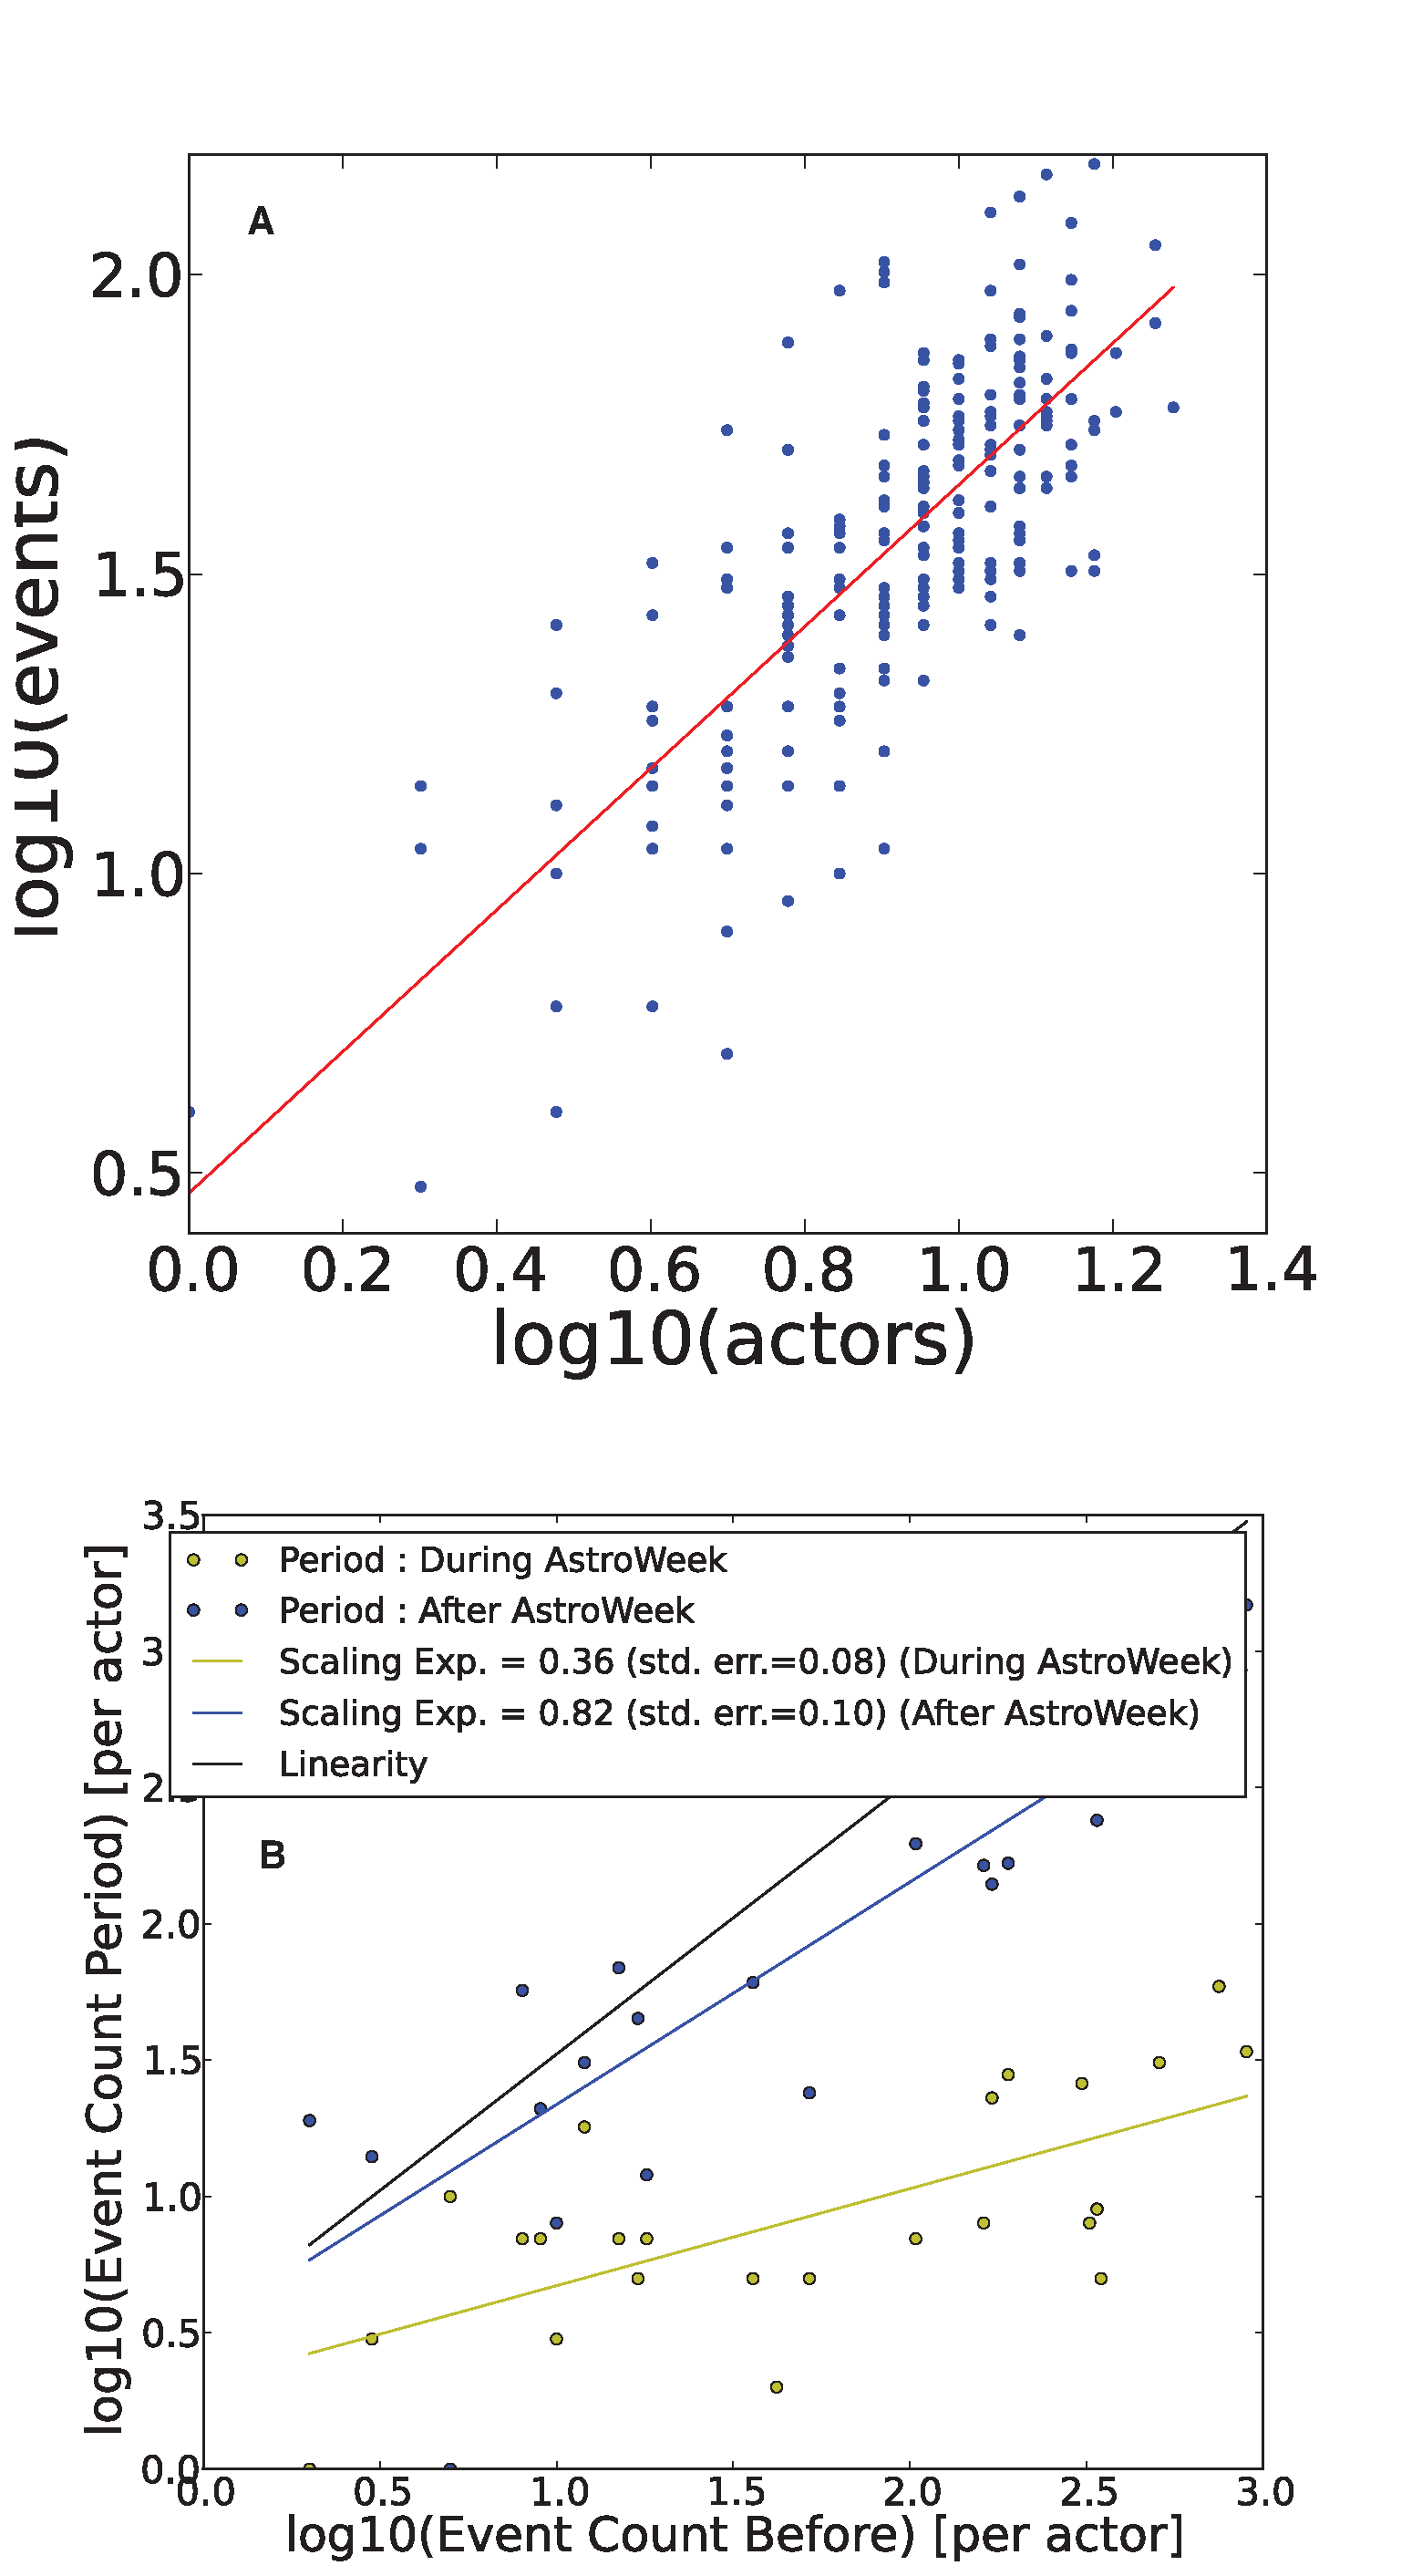
\includegraphics[width=0.9\columnwidth]{figures/tradeoff_senior_contributors.eps}
\caption{{\bf Panel A: } Count of events as a function of active actors per day (in double logarithmic scale). This relation exhibits a scaling given by equation \ref{eq:superlinear}, with exponent $\beta = 1.18 \pm 0.06$. After the Astro Hack Week the same relationship holds with exponent $1.18 \pm 0.07$ (not shown). {\bf Panel B: } Comparison of event counts per actor during and after the Astro Hack Week as a function of event count per actor before the hacking week. The amount of contributions exhibits a marginal decrease, characterized by the scaling exponent $\mu \approx 0.33 < 1$, i.e., following a sub-linear function of individual contributions during the Astro Hack Week as a function of individual contributions before. For reference, the count of contributions {\it after}  as a function of {\it before} the AstroWeek, is also presented, and appears to be very close to linearity (scaling exponent close to 1).}
\label{fig:tradeoff}
\end{figure}

Our results show that the Astro Hack Week had an {\it impulse} effect on the community, followed by mid-term and long-term spillovers, which can be measured precisely using the response function given by equation (\ref{eq:critical_decay}), with exponent $\alpha \approx 0.6$ larger (faster decay) for activity directly associated with the AstroWeek, and $\alpha \approx 0.25$ for activity indirectly related to AstroWeek projects. These results suggest that AstroWeek projects were rapidly abandoned and gave way to more heterogeneous contributions on GitHub, reflecting the increased exploration of the capabilities of open and reproducible science, by the actors having participated in the hackathon. The trade-offs faced by senior actors --when the teach instead of practicing open and reproducible science-- show that the community has undergone a punctual re-organization of the distribution of contributions during the Astro Hack Week.


%For example, taking a power law decay with exponent $\alpha = 0.25$, the remaining activity after $100$ (resp. $1000$) days, is $31.6\%$ (resp. $17.8\%$) of the initial peak activity. Note that with a larger power law exponent, such as $\alpha =0.60$ comparable to the decay of created repositories, the remaining activity is small after $100$ days  ($6.3\%$) and residual after $1000$ days ($1.5\%$). Thus, the value of the power law exponent $\alpha$ plays a critical role to measure the mid- and long-term after-effects of a punctual event, such as the Astro Hack Week.

%{\bf [add a study of events which are directly related to Astro Hack Week, versus peripheral events, (which by the way may be far more important)]}

%We distinguish three typical dynamics:
%- dynamics related to actions taken in relation with astro week (astro week actors, astro week repos)  (critical yet relatively short memory process)
%- dynamics related to actions taken by astro week actors, on indirectly related repositories (much longer memory process)  {\bf [check that the much longer memory process is not due to the addition of the latter to the former]}.
%- productive bursts, how they connect with the two former results, and how they offer a universal measure of the community, regardless of the exogenous Astro Hack Week event.

